%%%%%%%%%%%%%%%%%%%%%
%   AMS packages    %
%%%%%%%%%%%%%%%%%%%%%
\documentclass{beamer}
\usepackage{amsmath}
\usepackage{amsxtra}
\usepackage{amscd}
\usepackage{amsthm}
\usepackage{amsfonts}
\usepackage{amssymb}
\usepackage{eucal}
%\usepackage[all]{xy}
\usepackage{graphicx}
\usepackage{comment}
\usepackage{amssymb}
\usepackage{latexsym,amsmath,amscd,amssymb,epsfig,verbatim}
\usepackage{tikz}
\usetikzlibrary{arrows,shapes}

\newtheorem{thm}{Theorem}
\newtheorem{cor}[thm]{Corollary}
\newtheorem{lem}[thm]{Lemma}
\newtheorem{prop}[thm]{Proposition}
\newtheorem{ex}[thm]{Exercise}
\newtheorem{conjecture}{Conjecture}
%\newtheorem*{conjecture*}{Conjecture}

\theoremstyle{remark}
\newtheorem{rem}[thm]{Remark}
\newtheorem{eg}[thm]{Example}

%\newtheorem{counterexample}[thm]{Counterexample}
\newtheorem{defn}[thm]{Definition}
%\newtheorem{claim}[thm]{Claim}
%\newtheorem{note}[thm]{Notation}
%\newtheorem{warning}[thm]{Warning}
%\newtheorem{variant}[thm]{Variant}
%\newtheorem{question}[thm]{Question}
%\newtheorem{construction}[thm]{Construction}
%\newtheorem{terminology}[thm]{Terminology}
%\newtheorem{convention}[thm]{Convention}

\newcommand\nc{\newcommand}
\nc\on{\operatorname}
\nc\renc{\renewcommand}
\newcommand\ssec{\subsection}
\newcommand\sssec{\subsubsection}
\newcommand\bO{{\mathbf O}}
\newcommand\CC{{\mathcal C}}
\newcommand\BN{{\mathbb N}}
\newcommand\BC{{\mathbb C}}
\newcommand\BF{{\mathbb F}}
\newcommand\BR{{\mathbb R}}
\newcommand\BQ{{\mathbb Q}}
\newcommand\BBZ{{\mathbb Z}}
\newcommand\uR{\underline{R}}
\newcommand\uZ{\underline{\BBZ}}
\newcommand\CF{{\mathcal F}}
\newcommand\uCF{\underline{{\mathcal F}}}
\newcommand\BZ{{\mathbb Z}}
\newcommand\BA{{\mathbb A}}
\newcommand\BP{{\mathbb P}}
\newcommand\fa{{\mathfrak a}}
\newcommand\fp{{\mathfrak p}}
\newcommand\fq{{\mathfrak q}}
\newcommand\fm{{\mathfrak m}}
\newcommand\pt{\mathrm{pt}}
\newcommand\rk{\operatorname{rk}}
\newcommand\Aut{\operatorname{Aut}}




\newcommand\fbn{\mathcal H}
\newcommand \edgequot{\text{edge-quotient bijective }}

\def\Stab{\operatorname{Stab}}
\def\Fix{\operatorname{Fix}}
\newcommand\im{\text{Im}}


\AtBeginSection[]{
	\begin{frame}{Table of Contents}
		\tableofcontents[currentsection]
	\end{frame}
}

\mode<presentation>{}
\usetheme{PaloAlto}
\usecolortheme{seahorse}

%%%%%%%%%%%%   Title slide info  %%%%%%%%%%%%%
\title{Peckness of Edge Posets}
\author{David Hemminger, Aaron Landesman, Zijian Yao}

\begin{document}

%%%%%%%%%%%%  Title Frame  %%%%%%%%%%%%%%%%
\begin{frame}
	\titlepage
\end{frame}

%%%%%%%%%%%%%%%%%%%%   Section 1   %%%%%%%%%%%%%%%%%%%

\section{Background}






\begin{frame}{Basic Definitions}
\begin{defn}
Let $P$ be a finite graded poset of rank $n$, that is:
\begin{itemize}
\item Elements of $P$ are a disjoint union of $P_0,P_1,\ldots,P_n$, called the \textit{ranks}
\item If $x\in P_i$ and $x\lessdot y$, then $y\in P_{i+1}$
\item Define $\rk(x) = k$, where $x\in P_k$.
\end{itemize}
\end{defn}

\begin{defn}
A map $f\colon P\rightarrow Q$ is a \textit{morphism} from $P$ to $Q$ if $x\le_P y \implies f(x)\le_Q f(y)$ and $\rk(x) = \rk(f(x))$.  We say that $f$ is \textit{injective/surjective/bijective} if it is an injection/surjection/bijection from $P$ to $Q$ as sets.
\end{defn}
\end{frame}









\begin{frame}{Peck Posets}
\begin{defn}
Write $p_i = |P_i|$.  P is
\begin{itemize}

\item \textit{Rank-symmetric} if $p_i = p_{n-i}$ for all $1\le i\le n$

\item \textit{Rank-unimodal} if for some $0\le k\le n$ we have
$$p_0\le p_1\le \ldots \le p_k \ge p_{k+1} \ge\ldots \ge p_n$$

\item \textit{$k$-Sperner} if no disjoint union of $k$ antichains (sets of pairwise incomparable elements) in $P$ is larger than the disjoint union of the largest $k$ ranks of $P$

\item \textit{Strongly Sperner} if it is $k$-Sperner for all $1\le k\le n$.

\item \textit{Peck} if $P$ is rank-symmetric, rank-unimodal, and strongly Sperner.
\end{itemize}
\end{defn}
\end{frame}







\begin{frame}

\begin{defn}
Let $V(P)$ and $V(P_i)$ be the complex vector spaces with bases $\{x |x\in P\}$ and $\{x |x\in P_i\}$
\end{defn}

\begin{lem}[Stanley, 1980]
$P$ is Peck if and only if there exists an linear transformation $U\colon V(P)\rightarrow V(P)$ such that
\begin{itemize}
\item For every basis element $x\in P$, 
$$U(x) = \sum_{y\gtrdot x} c_{x,y}y$$

\item  For all $0\le i < \frac{n}{2}$, the map $U^{n-2i}\colon V(P_i)\rightarrow V(P_{n-i})$ is an isomorphism.
\end{itemize}
\end{lem}
\end{frame}







\begin{frame}
\begin{defn}
If the Lefschetz map defined by

$$L(x) = \sum_{y\gtrdot x} y$$

satisfies the second condition in the previous lemma, then $P$ is \textit{unitary Peck}.
\end{defn}
\end{frame}








\section{The Edge Poset and a Conjecture}

\begin{frame}{Definition of the Edge Poset}
\begin{defn}
\label{defn:functor_of_edges}
For $P$ a finite graded poset, it's \textit{edge poset} $\mathcal{E}(P)$ is the finite graded poset defined as follows. 
\begin{itemize}

\item Elements of $\mathcal{E}(P)$ are ordered pairs $(x,y)\in P\times P$ where $x\lessdot y$

\item Define $(x,y) \lessdot_{\mathcal{E}} (x^\prime,y^\prime)$ if $x\lessdot_P x^\prime$ and $y\lessdot_P y^\prime$

\item Define $\le_{\mathcal{E}}$ to be the transitive closure of $\lessdot_{\mathcal{E}}$

\item Define $\rk_{\mathcal{E}}(x,y) = \rk_P(x)$.
\end{itemize}
\end{defn}
\end{frame}







\begin{frame}
\begin{eg}
It is quite crucial we declare the relation $\leq_\mathcal F$ to be the transitive closure of $\lessdot_{\mathcal F}.$ An example of something that can go wrong is as follows. On the left hand side is the hasse diagram of a poset $P$ in the middle is the poset $\mathcal F^1(P)$ and on the right hand side is the poset obtained from the relation $x\otimes y \leq a\otimes b$ if $x \leq a, y \leq b.$

Here, it is clear that $\mathcal F^1(P)$ is a graded poset, with $rk(x\otimes y) = rk(x),$ but, the hasse diagram on the right represents a poset which does not have a grading.
\end{eg}

\end{frame}








\begin{frame}
\begin{center}
\begin{tikzpicture}[scale=.5] at (0,0)
  \node (0) at (0,0) {$0$};
  \node (1) at (-1,2) {$1$};
  \node (2) at (1,2) {$2$};
  \node (3) at (0,4) {$3$};
  \node (4) at (2,4) {$4$};
  \node (5) at (0,6) {$5$};
  \node (6) at (2,6) {$6$};
  \node (7) at (1,8) {$7$};
  \draw (0)--(1);
  \draw (0)--(2);
  \draw (1)--(3);
  \draw (2)--(3);
  \draw (2)--(4);
  \draw (3)--(5);
  \draw (4)--(6);
  \draw (5)--(7);
  \draw (6)--(7);
  \node (8) at (0,-2) {$P$};
\end{tikzpicture} \qquad
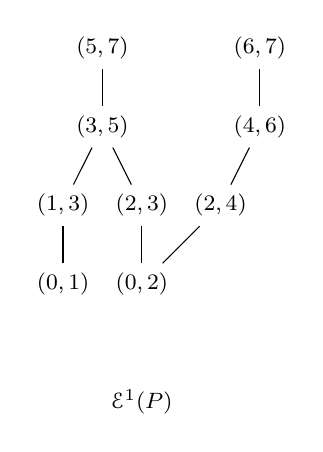
\begin{tikzpicture}[scale = .5]
  \node[font=\footnotesize] (0) at (0,1) {$(0,1)$};
  \node[font=\footnotesize] (1) at (2,1) {$(0,2)$};
  \node[font=\footnotesize] (2) at (0,3) {$(1,3)$};
  \node[font=\footnotesize] (3) at (2,3) {$(2,3)$};
  \node[font=\footnotesize] (4) at (4,3) {$(2,4)$};
  \node[font=\footnotesize] (5) at (1,5) {$(3,5)$};
  \node[font=\footnotesize] (6) at (5,5) {$(4,6)$};
  \node[font=\footnotesize] (7) at (1,7) {$(5,7)$};
  \node[font=\footnotesize] (8) at (5,7) {$(6,7)$};
  \draw (0)--(2);
  \draw (1)--(3);
  \draw (1)--(4);
  \draw (2)--(5);
  \draw (3)--(5);
  \draw (4)--(6);
  \draw (5)--(7);
  \draw (6)--(8);
  \node[font=\footnotesize] (9) at (2,-2) {$\mathcal E^1(P)$};
\end{tikzpicture} 
\end{center}
\end{frame}






\begin{frame}
\begin{center}
\begin{tikzpicture}[scale=.5] at (0,0)
  \node (0) at (0,0) {$0$};
  \node (1) at (-1,2) {$1$};
  \node (2) at (1,2) {$2$};
  \node (3) at (0,4) {$3$};
  \node (4) at (2,4) {$4$};
  \node (5) at (0,6) {$5$};
  \node (6) at (2,6) {$6$};
  \node (7) at (1,8) {$7$};
  \draw (0)--(1);
  \draw (0)--(2);
  \draw (1)--(3);
  \draw (2)--(3);
  \draw (2)--(4);
  \draw (3)--(5);
  \draw (4)--(6);
  \draw (5)--(7);
  \draw (6)--(7);
  \node (8) at (0,-2) {$P$};
\end{tikzpicture} \qquad
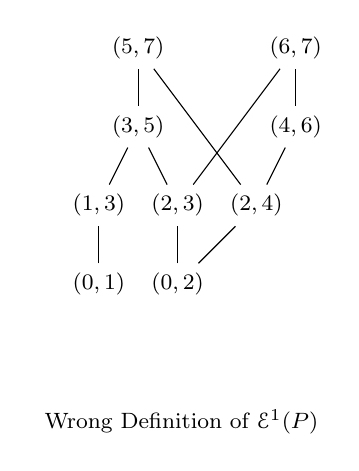
\begin{tikzpicture}[scale = .5]
  \node[font=\footnotesize] (0) at (0,1) {$(0,1)$};
  \node[font=\footnotesize] (1) at (2,1) {$(0,2)$};
  \node[font=\footnotesize] (2) at (0,3) {$(1,3)$};
  \node[font=\footnotesize] (3) at (2,3) {$(2,3)$};
  \node[font=\footnotesize] (4) at (4,3) {$(2,4)$};
  \node[font=\footnotesize] (5) at (1,5) {$(3,5)$};
  \node[font=\footnotesize] (6) at (5,5) {$(4,6)$};
  \node[font=\footnotesize] (7) at (1,7) {$(5,7)$};
  \node[font=\footnotesize] (8) at (5,7) {$(6,7)$};
  \draw (0)--(2);
  \draw (1)--(3);
  \draw (1)--(4);
  \draw (2)--(5);
  \draw (3)--(5);
  \draw (4)--(6);
  \draw (5)--(7);
  \draw (6)--(8);
  \draw (4)--(7);
  \draw (3)--(8);
  \node[font=\footnotesize] (9) at (2,-2.5) {$\text{ Wrong Definition of } \mathcal E^1(P)$};
\end{tikzpicture}
\end{center}
\end{frame}







\begin{frame}{A Conjecture on the Peckness of Edge Posets}
\begin{defn}
The \textit{boolean algebra of rank $n$} is the poset whose elements are subsets of $[n]$ with order given by containment, i.e. for $A,B\in B_n$, $A\le B$ if $A\subseteq B$.
\end{defn}

\begin{conjecture}[Hemminger, Landesman, and Yao 2014]
Let $G\subseteq \Aut(B_n)$.  Then $\mathcal{E}(B_n/G)$ is Peck.
\end{conjecture}
\end{frame}








\section{Main Result}
\subsection{Statement of Theorem}

\begin{frame}{Main Result}
\begin{defn}
A group action of $G$ on $P$ is \textit{cover transitive} if whenever $x,y,z\in P$ such that $x\lessdot z$, $y\lessdot z$, and $y\in Gx$, there exists some $g\in \Stab_G(z)$ such that $g\cdot x = y$.
\end{defn}

\begin{thm}[Hemminger, Landesman, and Yao 2014]
If a group action of $G$ on $B_n$ is cover transitive, then $\mathcal{E}(B_n/G)$ is Peck.
\end{thm}
\end{frame}






\subsection{Outline of Proof}

\begin{frame}
\begin{defn}
Given a group action of $G$ on $P$, we define a group action of $G$ on $\mathcal{E}(P)$ by letting $g\cdot (x,y) = (g\cdot x,g\cdot y)$ for all $g\in G$.
\end{defn}
\pause
\begin{prop}
The map $q\colon \mathcal{E}(P)/G\rightarrow \mathcal{E}(P/G)$ defined by $q(G(x,y)) = (Gx,Gy)$ is a surjective morphism.  Furthermore, $q$ is also injective if and only if the action of $G$ on $P$ is cover transitive.
\end{prop}

\begin{lem}
If $f:P\rightarrow Q$ is a bijective morphism and $P$ is Peck then $Q$ is Peck.
\end{lem}
\end{frame}







\begin{frame}
\begin{thm}[Stanley, 1984]
If $P$ is unitary Peck and $G\subseteq\operatorname{Aut}(P)$, then $P/G$ is Peck.
\end{thm}
It then suffices to show that $\mathcal{E}(B_n)$ is unitary Peck.  Unfortunately while this is true, the only proof that we know is long and computational.  Instead we outline a nicer --albeit less direct-- proof.
\end{frame}







\begin{frame}{Definition of $\mathcal{H}(P)$}
\begin{defn}
For $P$ a finite graded poset, define the graded poset $\mathcal H(P)$ as follows.
\begin{itemize}
\item Elements are pairs $(x,y)\in P\times P$ such that $x\lessdot y$

\item Define $(x,y) \lessdot_{\mathcal H} (x^\prime,y^\prime)$ if $x \lessdot_P x^\prime,y\lessdot_P y^\prime$ \textbf{and} $\mathbf{y \ne x^\prime}$

\item Define $\leq_{\mathcal H}$ to be the transitive closure of $\lessdot_{\mathcal H}$

\item Define $rk_{\mathcal H}(x,y) = rk_P(x).$
\end{itemize}
\end{defn}
\end{frame}









\begin{frame}{$\mathcal{H}(B_n)$ is unitary Peck}
add figure   %%% Which figure?
\end{frame}







\begin{frame}
\begin{defn}
As before, for $G$ acting on $P$, define $g\cdot (x,y) = (g\cdot x,g\cdot y)$.
\end{defn}

\begin{rem}
Since $\mathcal{E}(P)$ and $\mathcal{H}(P)$ have the same elements and $(x,y)\le_{\mathcal{H}} (x^\prime,y^\prime) \implies (x,y)\le_{\mathcal{E}} (x^\prime,y^\prime)$, there is a natural bijective morphism $\mathcal{H}(P)/G\rightarrow \mathcal{E}(P)/G$.
\end{rem}

\begin{proof}[Proof of Main Result]
$\mathcal{H}(B_n)$ unitary Peck $\implies \mathcal{H}(B_n)/G$ Peck $\implies \mathcal{E}(B_n)/G$ Peck $\implies \mathcal{E}(B_n/G)$ Peck.
\end{proof}
\end{frame}






\section{Cover Transitive Actions}

\begin{frame}{CCT actions}
\begin{lem}
\label{lem:cover_transitive_equivalence}
Let $G$ be a group acting on a graded poset $P.$ The following are equivalent:
\begin{enumerate}
	\item The action of $G$ on $P$ is CCT.
	\item Whenever $x \lessdot y,x \lessdot z,$ and $y \in Gz,$ there exists some $g \in Stab(x)$ with $gx = z.$
	\item The map $q\colon \mathcal E^r(P)/G\rightarrow \mathcal E^1(P/G)$ defined by $q(G(x, y)) = (Gx,Gy)$ is an bijective morphism (but not necessarily an isomorphism).
	\item The map $q\colon \mathcal E^r(P)/G\rightarrow \mathcal E^1(P/G)$ defined by $q(G(x, y)) = (Gx,Gy)$ is an injective morphism.
	\item For all $i$ there is an equality $|(\mathcal E^1(P)/G)_i|=| (\mathcal E^1(P/G))_i|$
\end{enumerate}
\end{lem}

\end{frame}





\begin{frame}{Some examples of CCT actions}

\end{frame}




\begin{frame}{The direct product}
\begin{thm}
\label{thm:direct_product_preservation}
For $\phi:G\times P\rightarrow P,\psi:H \times Q \rightarrow Q$ two CCT actions, then the direct product $\phi \times \psi:(G\times H)\times (P\times Q) \rightarrow (P\times Q),(g,h)\cdot (x,y) \mapsto (gx,hy)$ is also CCT.
\end{thm}
\end{frame}





\begin{frame}{The semi-direct product}
\begin{prop}\label{prop:semidirect_product_cover_transitive_actions}
Let $G\subseteq \operatorname{Aut}(P)$, $H\triangleleft G$, $K\subset G$ such that $G = H\rtimes K$.  Suppose that $H$ acts CC transitively on $P$ and $K$ acts CC transitively on $P/H$.  Then $G$ acts CC transitively on $P$.
\end{prop}
\end{frame}






\begin{frame}{The wreath product}
\begin{defn}
For $G, H$ groups, with $H \subset S_l,$ the {\it wreath product}, notated $G \wr H,$ is the group whose elements are pairs $(g,h) \in G^l\times H$ with multiplication defined by
\begin{align*}
((g_1',\ldots, g_l'),h') \cdot ((g_1,\ldots, g_l) ,h) =((g'_{h'(1)}g_1,\ldots, g'_{h'(l)}g_l),hh')
\end{align*}
where $h \in H$ acts on $[l]$ by the restriction of the permutation action of $S_l$ to $H.$
\end{defn}
\end{frame}



\begin{frame}{The wreath product}
\begin{thm}
\label{thm:wreath_preservation}
If $\psi:G\times P \rightarrow P$ is CCT, then $\phi:G\wr S_l \times P^l \rightarrow P^l$ where $\phi$ is the induced action is also CCT.
\end{thm}
\end{frame}



\begin{frame}{The automorphism of rooted trees}

\end{frame}





\begin{frame}{Automorphism of rooted trees}

\end{frame}






\begin{frame}{The Dihedral group $D_{2p}$ and $D_{4p}$}

\end{frame}







\section{Non CCT actions}
\begin{frame}{Unimodality of ranks of certain edge posets}


\end{frame}





\section{Some aspects of a $q$-analog}
\begin{frame}{The $q$ analog of the problem}

\end{frame}






\end{document}







